\documentclass[11pt,oneside]{book}
\usepackage[margin=1in]{geometry}
\usepackage[toc,page]{appendix}
\usepackage{graphicx}
\usepackage{natbib}
\usepackage{lipsum}
\usepackage{caption}
\usepackage{graphicx}

% disable chapter default name
\usepackage{titlesec}
\titleformat{\chapter}{\normalfont\huge}{\thechapter.}{20pt}{\huge}


% change the title of the table of contents
\renewcommand{\contentsname}{Indice}

% change the title of the list of images
\renewcommand{\contentsname}{Indice de imagens}

% paragraph spacing
\usepackage{indentfirst}
\setlength{\parindent}{3em}


\begin{document}

\captionsetup[figure]{margin=1.5cm,font=small,labelfont={bf},name={Figure},labelsep=colon,textfont={it}}
\captionsetup[table]{margin=1.5cm,font=small,labelfont={bf},name={Table},labelsep=colon,textfont={it}}
\setlipsumdefault{1}

\frontmatter

\begin{titlepage}


% -------------------------------------------------------------------
% You need to edit the details here
% -------------------------------------------------------------------

\begin{center}
{\LARGE Universidade de Aveiro}\\[7cm]
\linespread{1.2}\huge {\bfseries HW1: Mid-term assignment report }\\[0.5cm]
\linespread{1}
% \includegraphics[width=7.5cm]{images/soc.png}\\[1cm]
{\large{Pedro Miguel Nicolau Escaleira \textit{[88821]} }}\\[1cm]
\vspace*{\fill}
\large{15 de abril, 2020}
\end{center}

\end{titlepage}


% -------------------------------------------------------------------
% Contents
% -------------------------------------------------------------------

\tableofcontents

\listoffigures



% -------------------------------------------------------------------
% Main sections (as required)
% -------------------------------------------------------------------

\mainmatter

% !TEX root = ../main.tex

\chapter{Introdução}

\section{Contextualização do trabalho}
Este projeto, proposto pelo professor da disciplina de \textbf{Teste e Qualidade de Software}, teve como
principal objetivo a consolidação dos conhecimentos adquiridos durante as aulas da mesma tidas até ao momento.

Desta forma, foi sugerida a criação duma aplicação \textit{web} simples para obtenção de dados sobre a 
qualidade do ar num dado sitio fornecido. Para isso, a solução criada possui um \textit{back-end} sob a forma de 
\textit{REST API}, feita em \textit{java} com a ajuda de \textit{Spring Boot} e um \textit{fron-end} feito em 
\textit{python} com a ajuda de \textit{Flask} e \textit{Jinja 2}. Fazendo jus ao nome da disciplina, claramente
toda esta plataforma foi criada com o intuito de serem feitos testes, a vários níveis, para a mesma, pelo que foi,
duma forma geral, usado o \textit{JUnit} para a criação de testes para a \textit{api} e \textit{Selenium WebDriver}
para a criação de testes para a interface.

\section{Limitações}
Apesar do trabalho ter sido concluído com sucesso e de ter ido de encontro aos requisitos pedidos, 
houveram algumas \textit{features} que ficaram por implementar, mas que teriam sido uma adição que o autor
gostaria de ter criado. De seguida, são apresentadas as principais:

\begin{itemize}
   \item \textbf{Pesquisa dum lugar pelo nome}: no resultado final, apenas dá para pesquisar a qualidade de 
ar quando dadas as coordenadas da localização pretendida. Contudo, seria mais \textit{user friendly} fazer a mesma
pesquisa por nome.
   \item \textbf{Utilização doutra \textit{API} remota}: na solução final, apenas é usada um serviço remoto para
obtenção dos dados necessários. Contudo, tal como é sugerido nos pontos extra do guião do trabalho, seria mais
\textit{reliable} a utilização de mais que um serviço, para o caso do primeiro falhar. Esta aproximação não foi usada
já que iria adicionar uma grande quantidade de sobrecarga sobre o trabalho feito dada a dificuldade desta adição 
quando concluído grande parte do código feito.
   \item \textbf{Testes da interface em que houvesse alteração do código \textit{HTML}}: Seria algo de interesse de se
fazer testes, por exemplo, sob \textit{inputs} com atributos alterados, para testar o comportamento da plataforma
quando não apresentada, por exemplo, uma entrada na forma de número ou a submissão do formulário sem quaisquer 
\textit{inputs} obrigatórios preenchidos. Contudo, após alguma pesquisa, o \textit{Selenium IDE}, ferramenta usada
na criação dos testes da interface, não parece apresentar documentação de como fazer alterações no código fonte da
página testada.
\end{itemize}

% !TEX root = ../main.tex

\chapter{Especificações do produto}

\section{Funcionalidades e interações suportadas}
Como demonstrado na figura \ref{fig:interface_current}, esta plataforma é uma aplicação simples que permite aos seus 
utilizadores obterem a qualidade do ar para um determinado lugar, indicando as coordenadas. Permite não só
saber a qualidade atual, mas também a passada e futura. As métricas que ela disponibiliza são a \textbf{data 
referente à qualidade do ar}, o \textbf{valor escalar e textual da qualidade do ar}, o \textbf{poluente 
dominante} e a \textbf{concentração e valor escalar e textual da qualidade do ar referente a cada um dos
poluentes principais}.

\begin{figure}[h]
   \centering
   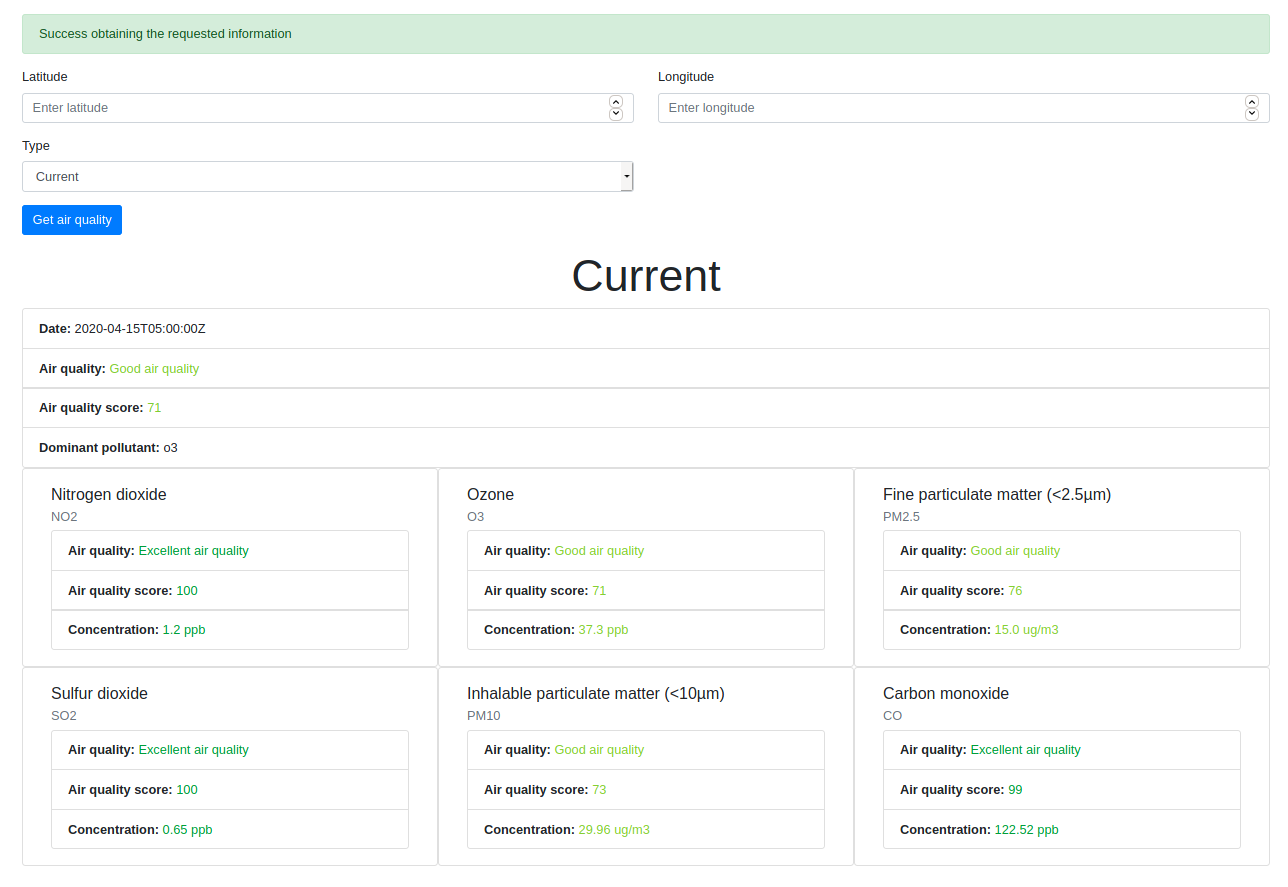
\includegraphics[width=0.90\textwidth]{images/interface_current}
   \caption{\textit{Print} da interface quando feito um pedido da qualidade do ar atual.}
   \label{fig:interface_current}
\end{figure}

Os possíveis utilizadores e cenários da plataforma criada são:

\begin{itemize}
   \item \textbf{População de risco}: dado o estado debilitado desta fração de população, é do interesse 
de algumas saber a qualidade do ar que respiram, principalmente as que possuem problemas respiratórios, 
de forma a melhor controlarem o seu estado de saúde. Desta forma, uma pessoa nestas condições poderá dirigir-se
à interface desta aplicação, introduzir as coordenadas do local onde se encontra ou se vai encontrar nos próximos
tempos, selecionar a obtenção de dados sobre o estado atual (\textit{Type Current}) ou sobre o estado previsto no 
futuro (\textit{Type Forecast}, selecionando também o número de horas seguintes sobre as quais pretende obter os 
dados) e, sendo assim, obter o estado da qualidade do ar atual ou nas horas seguintes, respetivamente.
   \item \textbf{Estudiosos}: profissionais que tenham interesse em estudar a qualidade de ar de acordo com 
o local, como por exemplo o estudo da evolução num determinado lugar. Sendo assim, um utilizador deste tipo
pode dirigir-se à página \textit{web}, selecionar um determinado lugar introduzindo as correspondentes coordenadas,
se pretende os dados de previsões passadas (\textit{Type History}) ou futuras (\textit{Type Forecast}) e o 
número de horas de dados deste o momento atual pretende obter. A partir dos resultados obtidos, poderá copiar
cada um deles e fazer o correspondente estudo.
\end{itemize}


\section{Arquitetura do sistema}
O \textit{back-end} do projeto foi feito usando \textit{java} com \textit{Maven} e \textit{Spring Boot}.
Quanto á arquitetura, é apresentado um diagrama de classes simples da mesma na figura 
\ref{fig:simple_diagram} (este diagrama de classes apenas contém as classes criadas e as relações entre elas,
sendo que os detalhes de cada uma se encontrarão definidos em diagramas expostos em subsecções seguintes, 
de forma a que este não fique demasiado confuso). Estas classes foram organizadas, de acordo com 
a sua complexidade em 4 \textit{packages}: \textbf{controller}, \textbf{model}, \textbf{serializers} e 
\textbf{service}. Nas subsecções seguintes

\begin{figure}[h]
   \centering
   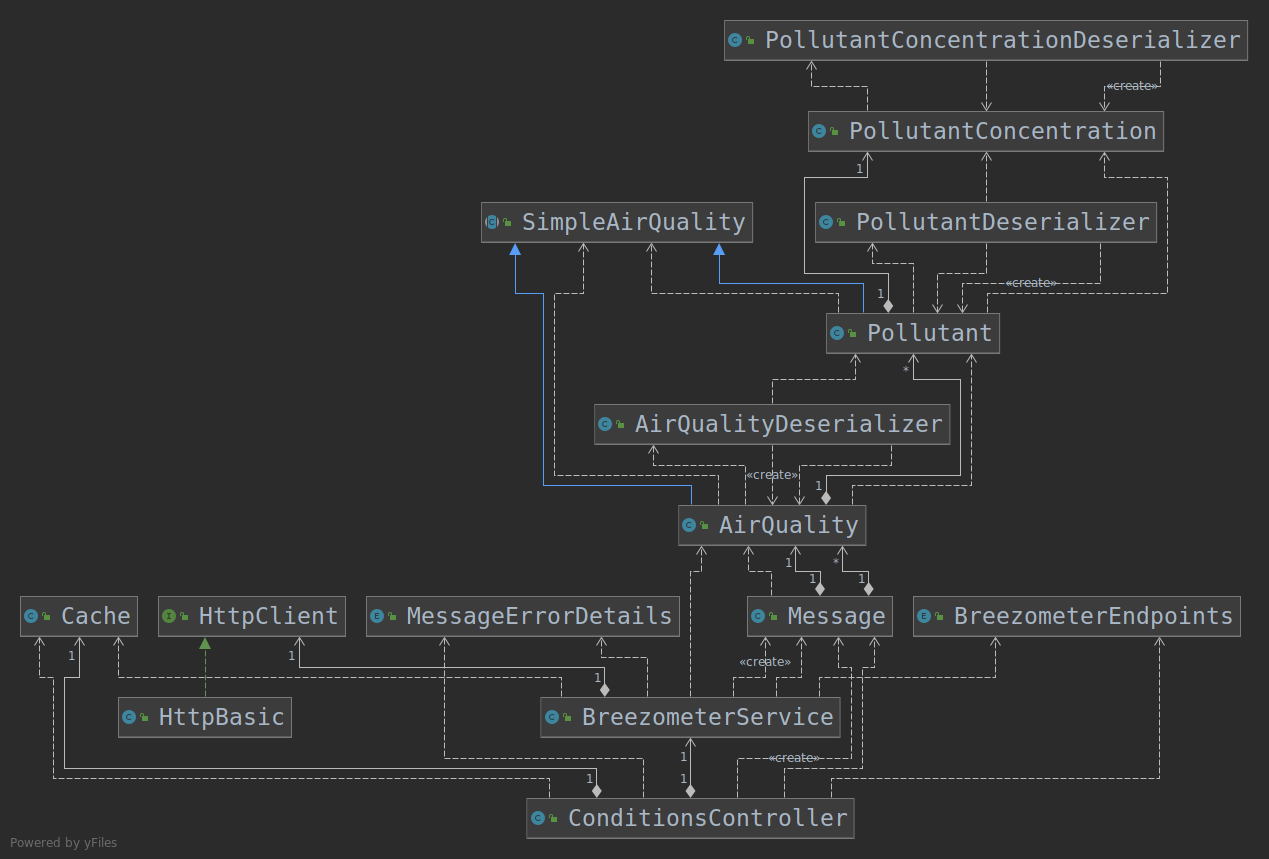
\includegraphics[width=0.90\textwidth]{images/simple_diagram}
   \caption{Diagrama de classes simples do projeto.}
   \label{fig:simple_diagram}
\end{figure}


\subsection{Package controller}
Este \textit{package} é constituído apenas por uma classe, \textbf{\textit{ConditionsController}}, que é
a responsável por lidar com as ligações feitas à \textit{API} criada. Desta forma, nesta classes são
definidos os \textit{endpoints} do nosso serviço e é definida a forma como cada \textit{request} vai ser
consumido no \textit{back-end}. Na figura \ref{fig:controller_diagram} é possível encontrar o esquema da
classe descrita.

\begin{figure}[h]
   \centering
   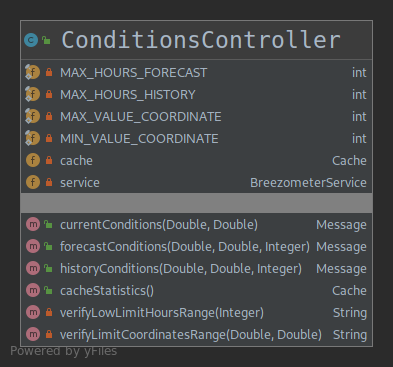
\includegraphics[width=0.40\textwidth]{images/controller_diagram}
   \caption{Diagrama das classes do \textit{package \textbf{controller}}.}
   \label{fig:controller_diagram}
\end{figure}


\subsection{Package model}
Todas as entidades usadas pelo nosso servido são representadas pelas classes deste \textit{package}. Desta forma, nela estão incluídas as classes:
\begin{itemize}
   \item \textbf{Que representam os dados da qualidade do ar}: 
      \begin{itemize}
         \item \textbf{\textit{AirQuality}}: representa a qualidade do ar referente a um determinado momento. Sendo assim, para além dos objetos desta classe possuírem informações básicas sobre a qualidade do ar, contêm também uma lista de poluentes (classe \textbf{\textit{Pollutant}}) que se encontram no ar no instante que esse objeto retrata.
         \item \textbf{\textit{Pollutant}}: classe que contém informações sobre um determinado poluente, como a forma como o respetivo poluente afeta a qualidade do ar e a concentração deste num determinado momento (classe \textbf{\textit{PollutantConcentration}}).
         \item \textbf{\textit{PollutantConcentration}}: classe que representa a informação da concentração dum poluente.
      \end{itemize}
   \item \textbf{Que modelam o sistema de cache}:
      \begin{itemize}
         \item \textbf{\textit{Cache}}: classe que permite criar objetos que simulam um sistema de cache simples e com as respetivas métricas (como o tamanho da cache ou o número de \textit{hits} e \textit{misses}). Por \textit{default}, os objetos de cache criados possuem um tamanho máximo determinado pelo valor da constante \textit{DEFAULT\_MAX\_SIZE}, sendo que quando o tamanho dela chega a esse tamanho máximo, os dados mais antigos são excluídos.
         \item \textbf{\textit{ParametersEncapsulation}}: classe que permite fazer o encapsulamento dos parâmetros sobre os quais se pretende armazenar a resposta dada pelo serviço externo na cache, isto é, quando é feito um pedido da qualidade do ar ao serviço externo, com uma determinada latitude, longidute, tipo de resposta (\textit{current}, \textit{history} ou \textit{forecast}) e possivelmente um número de horas, o resultado deste pedido pode ser armazenado na cache com um identificador representado pelo encapsulamento destes parâmetros.
      \end{itemize}
   \item \textbf{Ligadas às mensagens criadas pelo serviço}:
      \begin{itemize}
         \item \textbf{\textit{Message}}: classe que permite encapsular a resposta dada pela \textit{API} a um determinado pedido feito. Desta forma, ela tem um campo de sucesso, um de detalhes (para mensagens de sucesso ou erro), um da qualidade de ar (quando é feito um pedido da atual) e de uma lista de várias medições da qualidade do ar (quando é feito um pedido sobre os dados do passado ou futuro).
         \item \textbf{\textit{MessageErrorDetails}}: enumerável com as várias mensagens de erro que podem ser devolvidas pela mensagem enviada pela \textit{API}.
      \end{itemize}
\end{itemize}

Na figura \ref{fig:model_diagram} é possível verificar a constituição e relações entre cada uma destas classes.

\begin{figure}[h]
   \centering
   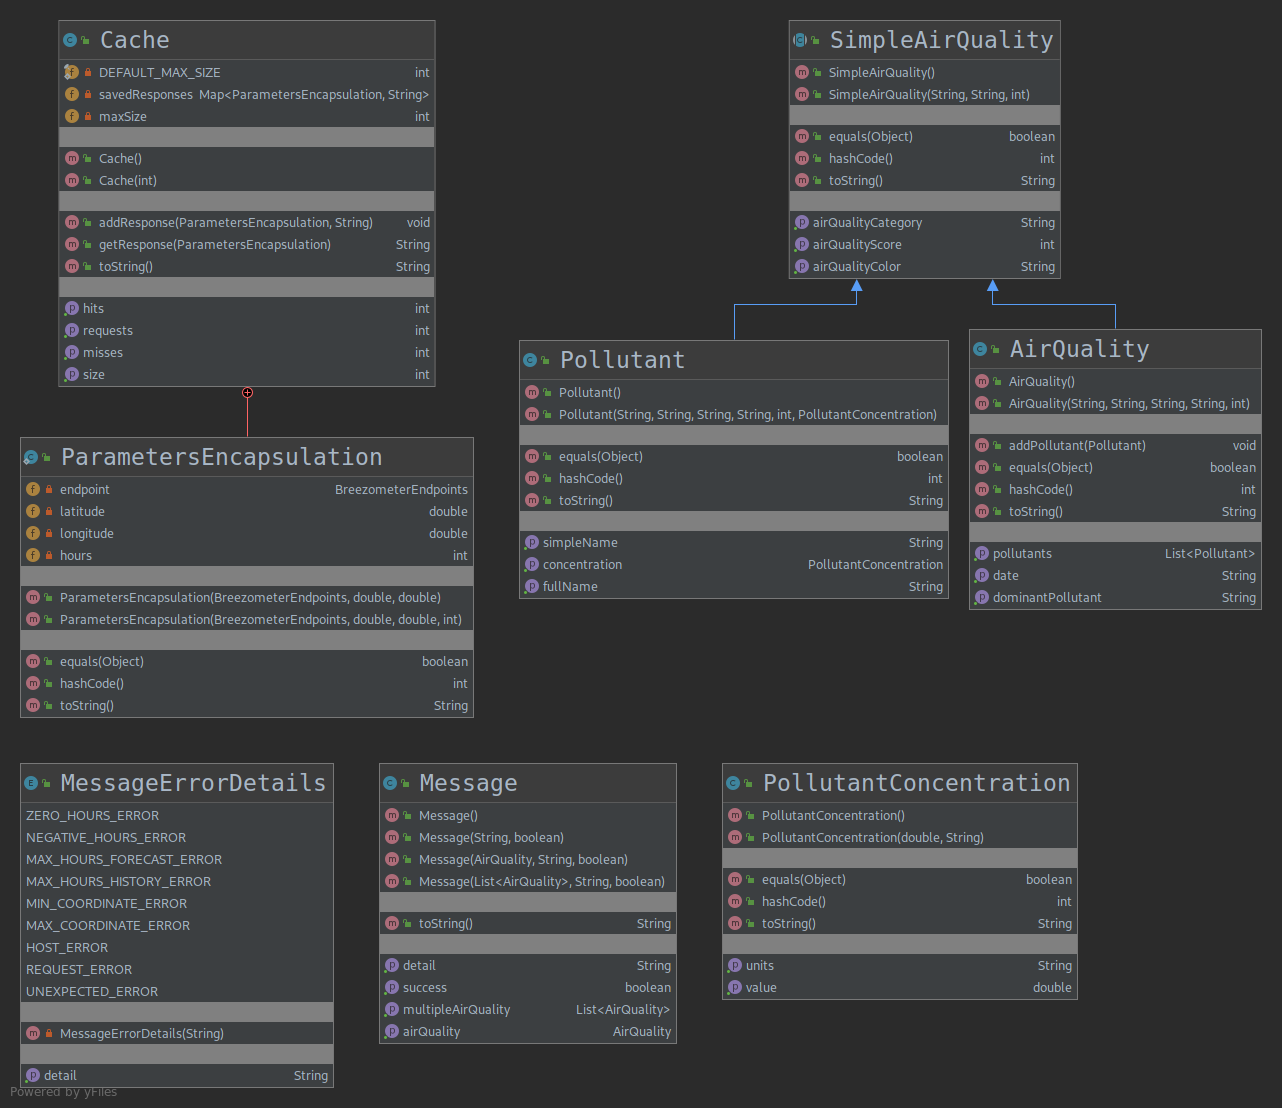
\includegraphics[width=0.90\textwidth]{images/model_diagram}
   \caption{Diagrama das classes do \textit{package \textbf{model}}.}
   \label{fig:model_diagram}
\end{figure}


\subsection{Package serializers}
De forma a poder fazer a "tradução" entre os dados recebidos do serviço externo e algumas das classes do \textit{model}, foram criados alguns \textit{deserializers} para esse efeito, como é possível verificar no diagrama da figura \ref{fig:serializers_diagram}. Para isso, foi usada a livraria \textit{Jackson}.
\begin{figure}[h]
   \centering
   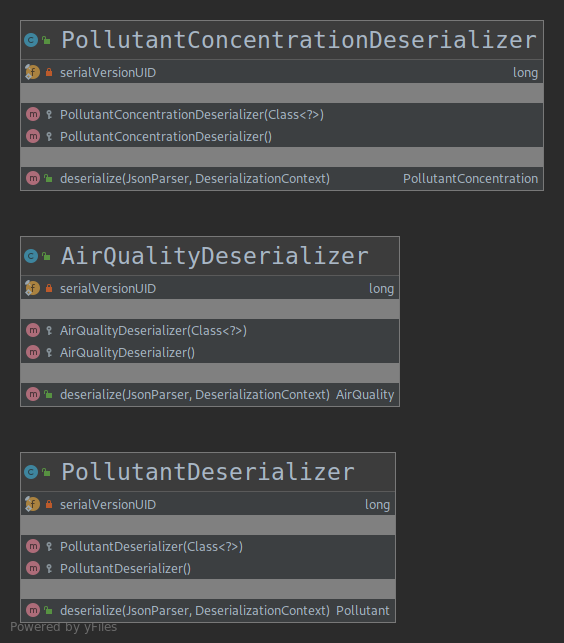
\includegraphics[width=0.90\textwidth]{images/serializers_diagram}
   \caption{Diagrama das classes do \textit{package \textbf{serializers}}.}
   \label{fig:serializers_diagram}
\end{figure}


\subsection{Package service}
De maneira a obter os dados necessários sobre a qualidade do ar, foi necessário criar um elo de ligação entre o \textit{back-end} criado e o serviço externo usado (\textit{BreezoMeter}), pelo que neste \textit{package} se encontram as classes que o permitem fazer. Quando a \textit{API} recebe um determinado pedido (excluindo o das estatísticas da cache), o método da classe \textbf{\textit{ConditionsController}} responsável por tratar do pedido "chama" o método \textit{requestApi} da classe \textbf{\textit{ConditionsController}} deste \textit{package} com o respetivo pedido, sendo que esta ultima faz um pedido ao serviço externo usando a classe \textbf{\textit{HttpBasic}} (disponibilizada pelo professor da disciplina numa das aulas práticas). A resposta do serviço externo é de seguida processada pelos \textit{deserializers} já descritos anteriormente e o objeto ou lista de objetos da classe \textbf{\textit{AirQuality}} são retornados ao método do \textit{controller} que tinha feito o pedido, encapsulados sob a forma dum objeto da classe \textbf{\textit{Message}}. Na figura \ref{fig:service_diagram} é possível encontrar a estrutura interna das classes deste \textit{package}.

\begin{figure}[h]
   \centering
   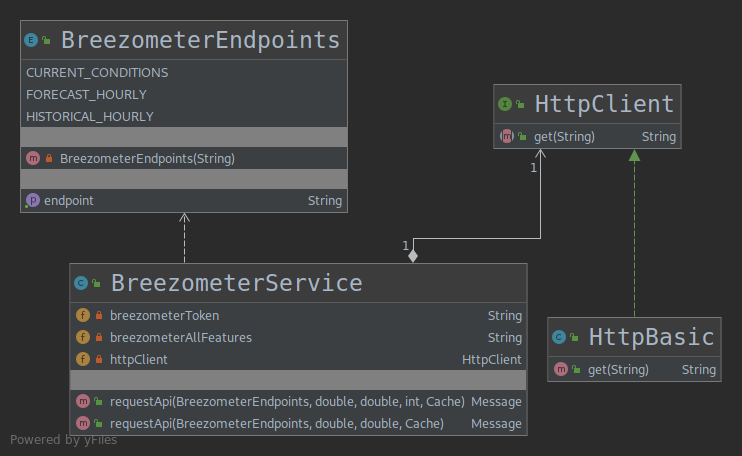
\includegraphics[width=0.90\textwidth]{images/service_diagram}
   \caption{Diagrama das classes do \textit{package \textbf{service}}.}
   \label{fig:service_diagram}
\end{figure}


\end{document}
